\documentclass[11pt, oneside]{article}
\usepackage[margin=1in]{geometry}
\geometry{letterpaper}
\usepackage{amssymb}
\usepackage[fleqn]{amsmath}
\usepackage[sharp]{easylist}
\usepackage{relsize}
\usepackage{graphicx}

\pagenumbering{gobble}              % No page numbering
\setlength{\parindent}{0em}         % No paragraph indenting
\setlength{\parskip}{0.5em}         % Paragraph spacing

\newcommand*{\begineasylist}{\begin{easylist}[itemize]\ListProperties(Style*=$\bullet$\quad, Style2*=\tiny$\blacksquare$\quad, Style3*=$\circ$\quad, Style4*=$\diamond$\quad, FinalSpace=1em, Space=0em, Space*=0em)}

\newcommand*{\begineasylistnumbered}{\begin{easylist}[enumerate]\ListProperties(Numbers=a, Space=0em, Space*=0em)}

\begin{document}

\section*{CS 349 Midterm Review}

\subsection*{Background \& History}
\begineasylist

# \textbf{User interface}: 
## The place where a person \emph{expresses intention} to an artifact, and the artifact \emph{presents feedback} to the person
## The way people (mental model) and technology (system model) interact

## Represented as MVC: \\
% \begin{figure}[h]
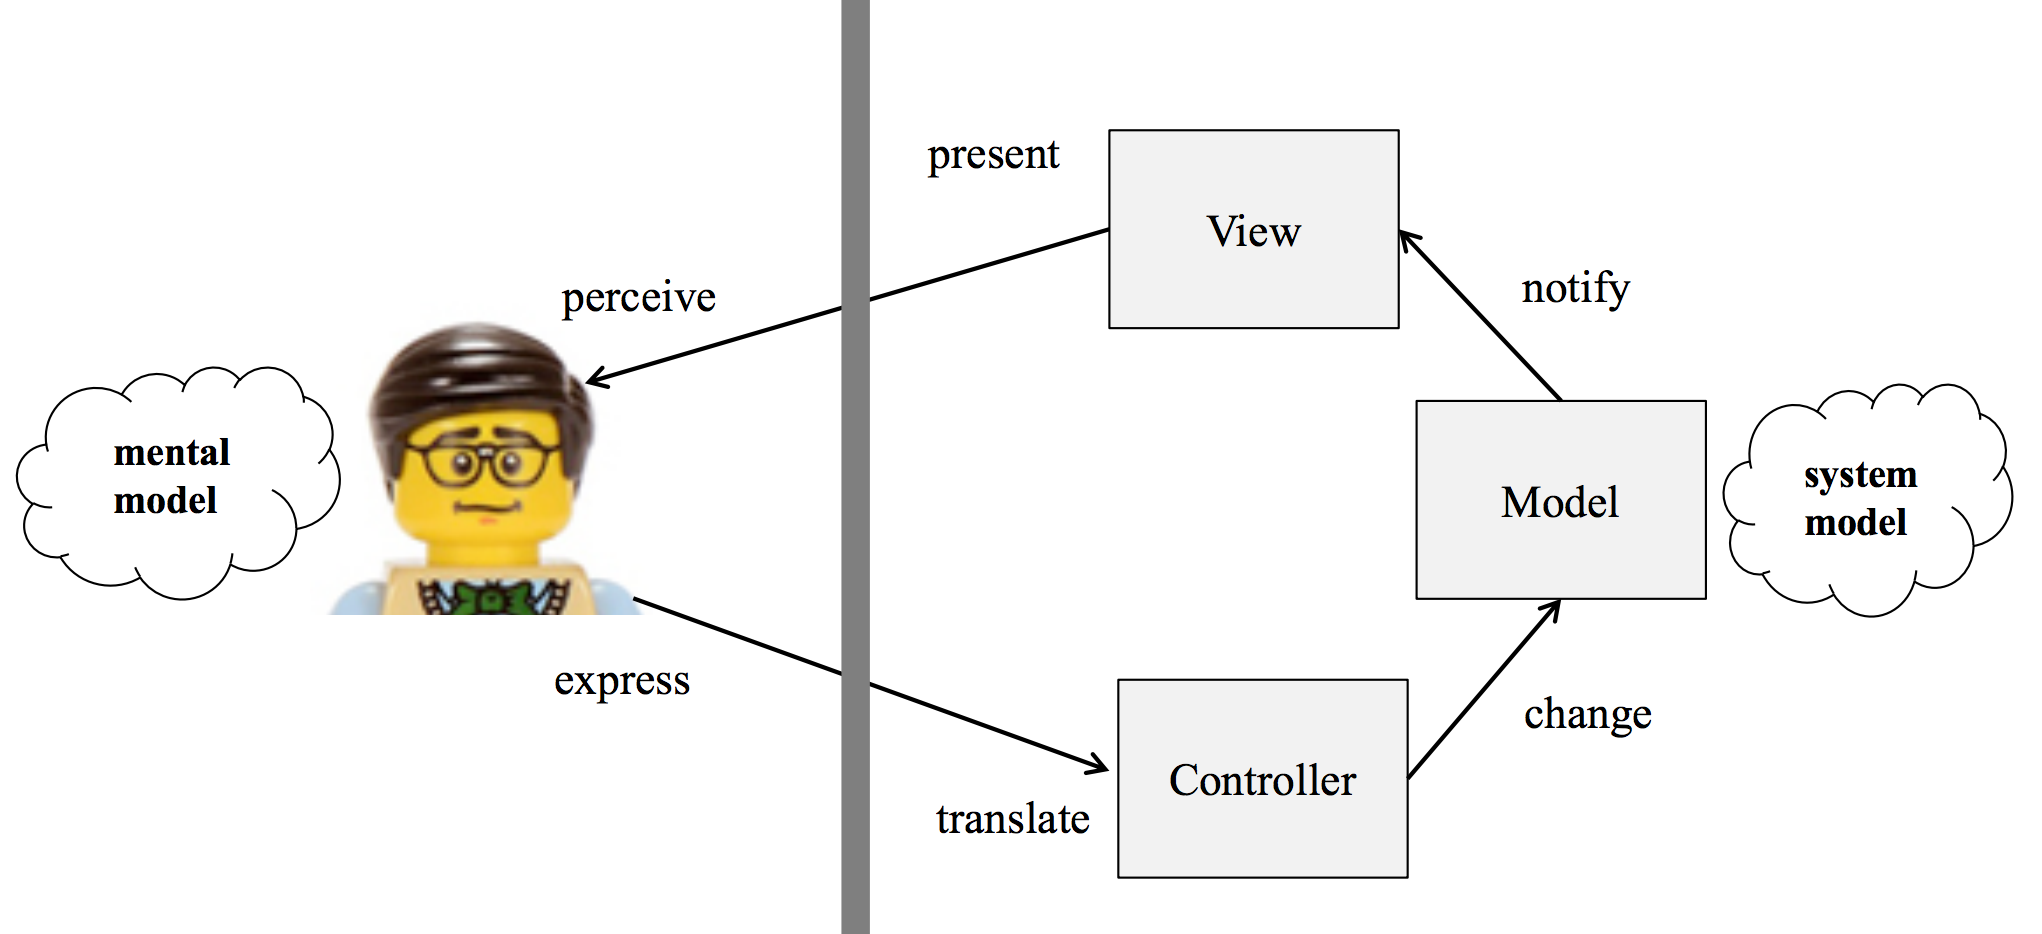
\includegraphics[width=0.7\textwidth]{res/intro_mvc.png}
% \end{figure}

# \textbf{Interface}: external presentation (visual, physical, auditory) to the user
## e.g. controls
# \textbf{Interaction}: actions invoked by user and corresponding responses (behaviour)
## e.g. action and dialog

# Batch interfaces (1945-1965)
## Sets of instructions fed via punch cards
## Only used by highly trained individuals

# Conversationalist interface (1965-1985+)
## Text-based feedback and input
## I/O is in system language, not task language

## Vannevar Bush -- created the memex, a desk with integrated display, input, and data storage
## Ivan Sutherland -- created the Sketchpad, an early graphical interface with a light pen and direct manipulation
## Douglas Engelbart -- invented the mouse, introduced copy/paste
## Alan Kay -- worked on the Xerox Star, first commercial computer with GUI

# Graphic user interface (1984+)
## Hardware interface: high resolution \& refresh graphics display, keyboard, and pointing device
## WIMP interface: windows, icons, menus, and pointer
## Benefits of GUI:
### Keeps the user in control
### Emphasize recognition (discovery of options) over recall (memorizing commands)
### Uses metaphor; makes interaction language closer to user's language

\end{easylist}

\subsection*{Windowing Systems \& X11}
\begineasylist

#

\end{easylist}

\subsection*{Java}
\begineasylist

#

\end{easylist}

\end{document}
